\documentclass[10pt,letterpaper]{article}

% Packages
\usepackage[margin=0.5in]{geometry}
\usepackage[utf8]{inputenc}
\usepackage[T1]{fontenc}
\usepackage{helvet}
\renewcommand{\familydefault}{\sfdefault}
\usepackage{xcolor}
\usepackage{tcolorbox}
\usepackage{array}
\usepackage{tabularx}
\usepackage{booktabs}
\usepackage{enumitem}
\usepackage{titlesec}
\usepackage{fancyhdr}
\usepackage{multicol}
\usepackage{graphicx}
\usepackage{tikz}
\usepackage{float}
\usetikzlibrary{shapes,arrows,positioning}

% Color definitions
\definecolor{headerblue}{RGB}{0,102,204}
\definecolor{stronggreen}{RGB}{0,153,76}
\definecolor{conditionalyellow}{RGB}{255,193,7}
\definecolor{researchblue}{RGB}{33,150,243}
\definecolor{warningred}{RGB}{204,0,0}
\definecolor{highlightgray}{RGB}{240,240,240}

% Section formatting - compact
\titleformat{\section}{\normalfont\fontsize{11}{12}\bfseries\color{headerblue}}{\thesection}{0.5em}{}
\titlespacing*{\section}{0pt}{4pt}{2pt}

\titleformat{\subsection}{\normalfont\fontsize{10}{11}\bfseries}{\thesubsection}{0.5em}{}
\titlespacing*{\subsection}{0pt}{3pt}{1pt}

% List formatting - ultra compact
\setlist[itemize]{leftmargin=*,itemsep=0pt,parsep=0pt,topsep=1pt}
\setlist[enumerate]{leftmargin=*,itemsep=0pt,parsep=0pt,topsep=1pt}

% Remove paragraph indentation
\setlength{\parindent}{0pt}
\setlength{\parskip}{2pt}

% Header/footer
\pagestyle{fancy}
\fancyhf{}
\fancyhead[L]{\footnotesize \textbf{Treatment Recommendations: EGFR-mutant Advanced NSCLC}}
\fancyhead[R]{\footnotesize Page \thepage}
\renewcommand{\headrulewidth}{0.5pt}
\fancyfoot[C]{\footnotesize Evidence-Based Clinical Guideline - For Professional Use Only}

\begin{document}

% Title block
\begin{center}
{\fontsize{14}{16}\selectfont\bfseries\color{headerblue} EVIDENCE-BASED TREATMENT RECOMMENDATIONS}\\[2pt]
{\fontsize{12}{14}\selectfont\bfseries Advanced/Metastatic Non-Small Cell Lung Cancer (NSCLC)}\\[2pt]
{\fontsize{11}{13}\selectfont\bfseries EGFR Exon 19 Deletion -- First-Line Therapy}\\[2pt]
{\fontsize{9}{11}\selectfont Version 1.0 | Effective Date: 2025-06-15 | Next Review: 2025-12-15}
\end{center}

\vspace{4pt}

% Recommendation Strength Legend
\begin{tcolorbox}[colback=highlightgray,colframe=black,title=\textbf{Recommendation Strength Key},fonttitle=\bfseries\small,coltitle=black]
{\small
\begin{itemize}
\item \colorbox{stronggreen!30}{\textbf{STRONG (Grade 1)}} - Benefits clearly outweigh risks; most patients should receive intervention
\item \colorbox{conditionalyellow!30}{\textbf{CONDITIONAL (Grade 2)}} - Trade-offs exist; shared decision-making essential
\item \colorbox{researchblue!30}{\textbf{RESEARCH (Grade R)}} - Insufficient evidence; clinical trial enrollment preferred
\end{itemize}

\textbf{Evidence Quality}: \textbf{A} = High (RCTs), \textbf{B} = Moderate (RCTs with limitations), \textbf{C} = Low (observational), \textbf{D} = Very low (expert opinion)
}
\end{tcolorbox}

\vspace{2pt}

\section{Clinical Context}

\subsection{Disease Overview}

Non-small cell lung cancer (NSCLC) accounts for approximately 85\% of all lung cancers and remains the leading cause of cancer-related mortality worldwide. Among NSCLC patients, activating mutations in the epidermal growth factor receptor (\textit{EGFR}) gene are identified in approximately 15--20\% of Caucasian and 40--50\% of East Asian patients with adenocarcinoma. The most common sensitizing \textit{EGFR} mutations are exon 19 deletions (approximately 45\% of \textit{EGFR}-mutant cases) and the L858R point mutation in exon 21 (approximately 40\%). These mutations confer sensitivity to EGFR tyrosine kinase inhibitors (TKIs), which have transformed the treatment paradigm and significantly improved progression-free survival (PFS) and overall survival (OS) compared with platinum-based chemotherapy.

\subsection{Patient Population}

\textbf{Target Population}:
\begin{itemize}
\item Adults $\geq$18 years with histologically confirmed advanced/metastatic NSCLC (Stage IIIB/IV)
\item Tumor harboring \textit{EGFR} exon 19 deletion (confirmed by NGS or validated PCR assay)
\item ECOG Performance Status 0--1 (this patient: ECOG PS 1)
\item First-line setting: No prior systemic anti-cancer therapy
\item No severe hepatic or renal impairment reported
\end{itemize}

\textbf{Exclusions/Caveats}:
\begin{itemize}
\item \textit{EGFR} exon 20 insertion mutations (distinct entity, not sensitive to standard EGFR TKIs)
\item Concurrent \textit{EGFR} T790M de novo resistance mutation (rare; requires osimertinib regardless)
\item ECOG PS $\geq$3 or life expectancy $<$3 months (supportive care may be more appropriate)
\item Severe interstitial lung disease (ILD) -- relative contraindication to EGFR TKIs
\item Uncontrolled brain metastases with significant mass effect (requires local therapy first)
\end{itemize}

\subsection{Biomarker Profile}

\textbf{Predictive Biomarker}: \textit{EGFR} exon 19 deletion
\begin{itemize}
\item \textbf{Type}: Activating (gain-of-function) mutation in the tyrosine kinase domain
\item \textbf{Mechanism}: In-frame deletion of amino acids 746--750 (most common variant: delE746-A750), resulting in constitutive EGFR kinase activation
\item \textbf{Detection Method}: Next-generation sequencing (NGS) preferred; PCR-based assays (e.g., Cobas\textregistered) also validated
\item \textbf{Clinical Significance}: Strong positive predictive biomarker for EGFR TKI response (ORR 60--80\%, median PFS 10--19 months depending on agent)
\item \textbf{Prognostic Value}: Exon 19 deletion associated with slightly better outcomes vs.~L858R on EGFR TKIs (subgroup analyses of FLAURA, ARCHER 1050)
\end{itemize}

\textbf{Additional Testing Recommended}:
\begin{itemize}
\item PD-L1 IHC (22C3 or SP263) -- informative but not required for treatment selection in \textit{EGFR}+ disease
\item Comprehensive NGS panel to assess co-mutations (\textit{TP53}, \textit{RB1}, \textit{PIK3CA}, \textit{MET} amplification)
\item Brain MRI with contrast (baseline staging; high CNS tropism in \textit{EGFR}+ NSCLC)
\end{itemize}

\section{Evidence Review}

\subsection{Key Clinical Trials}

\textbf{FLAURA Trial} (Soria et al., \textit{NEJM} 2018; Ramalingam et al., \textit{NEJM} 2020):
\begin{itemize}
\item \textbf{Design}: Phase 3, double-blind RCT, n=556, Osimertinib 80 mg QD vs.~1st-gen EGFR TKI (gefitinib or erlotinib)
\item \textbf{Population}: Treatment-na\"ive, \textit{EGFR} exon 19 del or L858R, advanced NSCLC, ECOG 0--1
\item \textbf{Primary Endpoint (PFS)}: 18.9 vs.~10.2 months (HR 0.46, 95\% CI 0.37--0.57, p$<$0.001)
\item \textbf{Overall Survival}: 38.6 vs.~31.8 months (HR 0.80, 95\% CI 0.64--1.00, p=0.046)
\item \textbf{ORR}: 80\% vs.~76\%; \textbf{DOR}: 17.2 vs.~8.5 months
\item \textbf{CNS Efficacy}: CNS PFS not reached vs.~13.9 months (HR 0.48); CNS ORR 66\% vs.~27\% in patients with measurable CNS lesions
\item \textbf{Safety}: Grade $\geq$3 AEs 34\% vs.~45\%; discontinuation due to AEs 13\% vs.~18\%
\item \textbf{Quality}: \textbf{High} -- large RCT, low risk of bias, adequate power, ITT analysis, crossover-adjusted OS
\item \textbf{Exon 19 Del Subgroup}: PFS HR 0.38; OS HR 0.68 -- greater benefit than L858R subgroup
\end{itemize}

\textbf{FLAURA2 Trial} (Planchard et al., \textit{NEJM} 2023):
\begin{itemize}
\item \textbf{Design}: Phase 3, open-label RCT, n=586, Osimertinib + platinum-pemetrexed chemotherapy vs.~Osimertinib alone
\item \textbf{Population}: Treatment-na\"ive, \textit{EGFR} exon 19 del or L858R, advanced NSCLC
\item \textbf{Primary Endpoint (PFS)}: 25.5 vs.~16.7 months (HR 0.62, 95\% CI 0.49--0.79, p$<$0.001)
\item \textbf{ORR}: 83\% vs.~76\%; \textbf{DOR}: 24.0 vs.~16.6 months
\item \textbf{CNS Efficacy}: CNS PFS HR 0.47; improved intracranial control with combination
\item \textbf{Safety}: Grade $\geq$3 AEs 64\% vs.~27\%; chemotherapy-related toxicity (nausea, cytopenias) added to TKI profile
\item \textbf{Quality}: \textbf{High} -- large RCT, open-label design (potential bias), mature PFS, OS data immature
\end{itemize}

\textbf{MARIPOSA Trial} (Cho et al., \textit{Lancet Oncol} 2024):
\begin{itemize}
\item \textbf{Design}: Phase 3, randomized, n=858, Amivantamab + Lazertinib vs.~Osimertinib
\item \textbf{Population}: Treatment-na\"ive, \textit{EGFR} exon 19 del or L858R, advanced NSCLC
\item \textbf{Primary Endpoint (PFS)}: 23.7 vs.~16.6 months (HR 0.70, 95\% CI 0.58--0.85, p$<$0.001)
\item \textbf{ORR}: 86\% vs.~79\%; \textbf{DOR}: 20.1 vs.~15.3 months
\item \textbf{Safety}: Grade $\geq$3 AEs 75\% vs.~43\%; infusion-related reactions with amivantamab (74\%, mostly grade 1--2)
\item \textbf{Quality}: \textbf{Moderate-High} -- large RCT, OS data immature, higher toxicity profile
\end{itemize}

\textbf{ARCHER 1050} (Soria et al., \textit{Lancet Oncol} 2018; Ramalingam et al., \textit{JCO} 2020):
\begin{itemize}
\item \textbf{Design}: Phase 3, open-label RCT, n=452, Dacomitinib vs.~Gefitinib
\item \textbf{Primary Endpoint (PFS)}: 14.7 vs.~9.2 months (HR 0.59, 95\% CI 0.47--0.74, p$<$0.001)
\item \textbf{Overall Survival}: 34.1 vs.~26.8 months (HR 0.71, 95\% CI 0.55--0.92, p=0.017)
\item \textbf{Exon 19 Del Subgroup}: OS HR 0.61 -- favorable
\item \textbf{Safety}: Grade $\geq$3 AEs 63\% vs.~31\%; diarrhea (8\% grade 3), rash/acne (14\% grade 3)
\item \textbf{Quality}: \textbf{Moderate} -- open-label, no CNS efficacy data (excluded brain metastases)
\end{itemize}

\subsection{Guideline Concordance}

\begin{table}[H]
\centering
\small
\begin{tabular}{p{3cm}p{8cm}p{3.5cm}}
\toprule
\textbf{Guideline} & \textbf{Recommendation} & \textbf{Evidence Level} \\
\midrule
NCCN v3.2025 & Osimertinib preferred first-line for \textit{EGFR} exon 19 del/L858R; Osimertinib + chemo also Category 1 & Category 1 (preferred) \\
ASCO 2024 & Osimertinib recommended as standard first-line; combination with chemo may be considered & Strong, Evidence A \\
ESMO 2024 & Osimertinib standard of care; Osimertinib + chemo option for high-risk patients & Grade I, A (ESMO-MCBS 4) \\
CSCO 2024 & Osimertinib preferred (I-level); Amivantamab + Lazertinib as alternative (II-level) & Level I recommendation \\
\bottomrule
\end{tabular}
\caption{Major guideline recommendations for first-line EGFR-mutant NSCLC}
\end{table}

\section{Treatment Options}

\subsection{First-Line Therapy}

\vspace{3pt}

\begin{tcolorbox}[enhanced,colback=stronggreen!10,colframe=stronggreen,
title={\textbf{Option 1: Osimertinib Monotherapy} \hfill \colorbox{white}{\textbf{STRONG (1A)}}},
fonttitle=\bfseries\small,coltitle=black]
{\small
\textbf{Regimen}:
\begin{itemize}
\item Osimertinib: 80 mg orally once daily
\item Duration: Until disease progression or unacceptable toxicity
\item Dose modifications: Reduce to 40 mg QD for severe toxicity; interrupt for $\leq$3 weeks if needed
\end{itemize}

\textbf{Evidence Basis}:
\begin{itemize}
\item Primary study: FLAURA trial, n=556
\item Primary outcome: PFS 18.9 vs.~10.2 months (HR 0.46, p$<$0.001); OS 38.6 vs.~31.8 months (HR 0.80, p=0.046)
\item ORR: 80\%; DOR: 17.2 months
\item Exon 19 del subgroup: PFS HR 0.38; OS HR 0.68 -- greater benefit magnitude
\item CNS efficacy: CNS PFS HR 0.48; CNS ORR 66\% in patients with measurable brain lesions
\end{itemize}

\textbf{Indications}:
\begin{itemize}
\item \textit{EGFR} exon 19 deletion or L858R mutation-positive advanced NSCLC
\item ECOG PS 0--1 (also used in PS 2 with caution)
\item Suitable for patients with or without baseline CNS metastases
\end{itemize}

\textbf{Key Toxicities}:
\begin{itemize}
\item Grade $\geq$3 AEs: 34\% (vs.~45\% with 1st-gen TKI)
\item Common: Diarrhea (58\%, 4\% grade 3), rash (58\%, 1\% grade 3), dry skin (36\%), paronychia (35\%)
\item Serious: QTc prolongation (monitor if risk factors), ILD/pneumonitis (3.9\%, potentially fatal), cardiomyopathy (LVEF decrease)
\item Discontinuation due to AEs: 13\%
\item Management: Supportive care for skin/GI AEs; dose interrupt/reduce for grade $\geq$3; permanent discontinuation for confirmed ILD
\end{itemize}

\textbf{Monitoring}:
\begin{itemize}
\item Baseline: ECG (QTc), LVEF (echocardiogram or MUGA), LFTs, renal function
\item Ongoing: LFTs and CBC every 3 months; ECG if symptoms or risk factors; imaging every 8--12 weeks (RECIST v1.1)
\item CNS monitoring: Brain MRI at baseline and if neurological symptoms develop
\item Clinical assessment: Every 4--8 weeks
\end{itemize}

\textbf{Recommendation Strength}: \textbf{STRONG} -- Benefits clearly outweigh risks\\
\textbf{Evidence Quality}: \textbf{HIGH} -- Well-designed RCT with consistent results, OS benefit confirmed
}
\end{tcolorbox}

\vspace{3pt}

\begin{tcolorbox}[enhanced,colback=conditionalyellow!10,colframe=conditionalyellow,
title={\textbf{Option 2: Osimertinib + Platinum-Pemetrexed Chemotherapy} \hfill \colorbox{white}{\textbf{CONDITIONAL (1B)}}},
fonttitle=\bfseries\small,coltitle=black]
{\small
\textbf{Regimen}:
\begin{itemize}
\item Osimertinib: 80 mg orally once daily (continuous)
\item Carboplatin: AUC 5 IV Day 1 (or Cisplatin 75 mg/m$^2$ IV Day 1)
\item Pemetrexed: 500 mg/m$^2$ IV Day 1
\item Chemotherapy: Every 3 weeks for 4 cycles, then osimertinib maintenance
\item Vitamin B12 and folic acid supplementation required with pemetrexed
\end{itemize}

\textbf{Evidence Basis}:
\begin{itemize}
\item Primary study: FLAURA2 trial, n=586
\item Primary outcome: PFS 25.5 vs.~16.7 months (HR 0.62, p$<$0.001) vs.~osimertinib alone
\item ORR: 83\%; DOR: 24.0 months
\item CNS PFS HR 0.47 -- enhanced intracranial control
\item OS data immature at time of publication
\end{itemize}

\textbf{Indications}:
\begin{itemize}
\item \textit{EGFR} exon 19 deletion or L858R advanced NSCLC
\item Consider for patients with high-risk features: high tumor burden, brain metastases, \textit{TP53} co-mutation, or aggressive disease
\item ECOG PS 0--1 with adequate organ function for chemotherapy
\end{itemize}

\textbf{Key Toxicities}:
\begin{itemize}
\item Grade $\geq$3 AEs: 64\% (vs.~27\% osimertinib alone)
\item Chemotherapy-related: Nausea (42\%), neutropenia (28\%, 13\% grade 3--4), anemia (23\%), fatigue (22\%)
\item TKI-related: Diarrhea, rash, QTc prolongation (as above)
\item Febrile neutropenia: $\sim$5\%
\item Discontinuation of chemotherapy component: $\sim$30\% (most continued osimertinib)
\end{itemize}

\textbf{Monitoring}:
\begin{itemize}
\item During chemotherapy phase: CBC before each cycle; renal function (cisplatin/carboplatin); LFTs
\item Ongoing TKI monitoring: As for Option 1
\item Imaging: Every 6--8 weeks during chemotherapy, then every 8--12 weeks on maintenance
\end{itemize}

\textbf{Recommendation Strength}: \textbf{CONDITIONAL} -- PFS benefit clear but added toxicity; OS not yet confirmed\\
\textbf{Evidence Quality}: \textbf{MODERATE-HIGH} -- Large RCT, open-label, mature PFS, OS immature
}
\end{tcolorbox}

\vspace{3pt}

\begin{tcolorbox}[enhanced,colback=conditionalyellow!10,colframe=conditionalyellow,
title={\textbf{Option 3: Amivantamab + Lazertinib} \hfill \colorbox{white}{\textbf{CONDITIONAL (1B)}}},
fonttitle=\bfseries\small,coltitle=black]
{\small
\textbf{Regimen}:
\begin{itemize}
\item Lazertinib: 80 mg orally once daily
\item Amivantamab: 1050 mg IV weekly for Weeks 1--4, then every 2 weeks (first infusion split over Days 1--2 to mitigate infusion reactions)
\item Duration: Until disease progression or unacceptable toxicity
\item Premedication: Diphenhydramine, acetaminophen, and corticosteroid before amivantamab infusions
\end{itemize}

\textbf{Evidence Basis}:
\begin{itemize}
\item Primary study: MARIPOSA trial, n=858
\item Primary outcome: PFS 23.7 vs.~16.6 months (HR 0.70, p$<$0.001) vs.~osimertinib
\item ORR: 86\%; DOR: 20.1 months
\item OS data immature
\end{itemize}

\textbf{Indications}:
\begin{itemize}
\item \textit{EGFR} exon 19 deletion or L858R advanced NSCLC (FDA/EMA regulatory status pending as of mid-2025)
\item Consider when IV therapy is feasible and patient tolerates infusion schedule
\item May be advantageous for patients with high disease burden or CNS involvement
\end{itemize}

\textbf{Key Toxicities}:
\begin{itemize}
\item Grade $\geq$3 AEs: 75\% (vs.~43\% osimertinib alone)
\item Infusion-related reactions: 74\% (mostly grade 1--2; 2\% grade $\geq$3)
\item Rash/acneiform dermatitis (common, EGFR class effect + amivantamab)
\item VTE: 9\% (higher than osimertinib alone)
\item Paronychia, stomatitis, diarrhea
\item Discontinuation due to AEs: higher than osimertinib monotherapy
\end{itemize}

\textbf{Monitoring}:
\begin{itemize}
\item Infusion monitoring: Vital signs during and 1 hour post-infusion; observe for infusion reactions
\item VTE surveillance: Monitor for DVT/PE symptoms; consider prophylaxis in high-risk patients
\item Skin toxicity: Proactive dermatologic management
\item Imaging: Every 8--12 weeks
\end{itemize}

\textbf{Recommendation Strength}: \textbf{CONDITIONAL} -- PFS benefit demonstrated but higher toxicity; OS immature; regulatory approval status varies\\
\textbf{Evidence Quality}: \textbf{MODERATE-HIGH} -- Large RCT, open-label comparator, OS not yet mature
}
\end{tcolorbox}

\vspace{3pt}

\begin{tcolorbox}[enhanced,colback=conditionalyellow!10,colframe=conditionalyellow,
title={\textbf{Option 4: Dacomitinib Monotherapy} \hfill \colorbox{white}{\textbf{CONDITIONAL (2B)}}},
fonttitle=\bfseries\small,coltitle=black]
{\small
\textbf{Regimen}:
\begin{itemize}
\item Dacomitinib: 45 mg orally once daily
\item Duration: Until disease progression or unacceptable toxicity
\item Dose reductions: 30 mg $\rightarrow$ 15 mg for toxicity
\end{itemize}

\textbf{Evidence Basis}:
\begin{itemize}
\item Primary study: ARCHER 1050, n=452
\item PFS: 14.7 vs.~9.2 months (HR 0.59, p$<$0.001) vs.~gefitinib
\item OS: 34.1 vs.~26.8 months (HR 0.71, p=0.017)
\item Exon 19 del subgroup: OS HR 0.61
\item No CNS efficacy data (patients with brain metastases excluded)
\end{itemize}

\textbf{Indications}:
\begin{itemize}
\item \textit{EGFR} exon 19 del or L858R advanced NSCLC
\item Consider when osimertinib is unavailable or cost-prohibitive
\item Not recommended if CNS metastases present (no efficacy data in this population)
\end{itemize}

\textbf{Key Toxicities}:
\begin{itemize}
\item Grade $\geq$3 AEs: 63\% (vs.~31\% gefitinib)
\item Diarrhea (87\%, 8\% grade 3), rash/acneiform dermatitis (69\%, 14\% grade 3), paronychia (62\%), stomatitis (44\%, 4\% grade 3)
\item Higher rate of dose reductions ($\sim$66\%) and treatment discontinuations due to AEs
\end{itemize}

\textbf{Monitoring}:
\begin{itemize}
\item Proactive skin and GI toxicity management (prophylactic minocycline, moisturizers, loperamide)
\item LFTs, CBC every 4--8 weeks
\item Imaging every 8--12 weeks
\end{itemize}

\textbf{Recommendation Strength}: \textbf{CONDITIONAL} -- OS benefit demonstrated but higher toxicity and no CNS data\\
\textbf{Evidence Quality}: \textbf{MODERATE} -- Open-label trial, excluded CNS metastases, older comparator
}
\end{tcolorbox}

\vspace{3pt}

\begin{tcolorbox}[enhanced,colback=highlightgray,colframe=black,
title={\textbf{Option 5: Gefitinib / Erlotinib (1st-Generation EGFR TKI)} \hfill \colorbox{white}{\textbf{NOT PREFERRED (2B)}}},
fonttitle=\bfseries\small,coltitle=black]
{\small
\textbf{Regimen}:
\begin{itemize}
\item Gefitinib: 250 mg orally once daily, OR
\item Erlotinib: 150 mg orally once daily (fasting)
\item Duration: Until disease progression or unacceptable toxicity
\end{itemize}

\textbf{Evidence Basis}:
\begin{itemize}
\item Multiple Phase 3 trials (IPASS, EURTAC, OPTIMAL, ENSURE) demonstrate PFS benefit vs.~chemotherapy
\item Median PFS: 9--13 months; ORR: 60--74\%
\item Inferior PFS and OS compared with osimertinib (FLAURA) and dacomitinib (ARCHER 1050)
\item High rate of acquired T790M resistance ($\sim$60\%), which can be addressed with second-line osimertinib
\end{itemize}

\textbf{Role in Current Practice}:
\begin{itemize}
\item Acceptable only when newer-generation TKIs are unavailable (resource-limited settings, insurance restrictions)
\item Sequential strategy (1st-gen TKI $\rightarrow$ T790M testing $\rightarrow$ osimertinib) may achieve comparable cumulative PFS in selected patients, but requires re-biopsy and risks missing the T790M window
\end{itemize}

\textbf{Recommendation Strength}: \textbf{CONDITIONAL AGAINST} -- Inferior to osimertinib; use only when preferred options unavailable\\
\textbf{Evidence Quality}: \textbf{MODERATE} -- High-quality trials but superseded by newer agents
}
\end{tcolorbox}

\vspace{3pt}

\subsection{Treatment Selection Summary}

\begin{table}[H]
\centering
\small
\begin{tabular}{p{3.5cm}p{1.8cm}p{2.2cm}p{1.5cm}p{2.5cm}p{2.5cm}}
\toprule
\textbf{Regimen} & \textbf{mPFS (mo)} & \textbf{mOS (mo)} & \textbf{Grade $\geq$3 AE} & \textbf{CNS Activity} & \textbf{GRADE} \\
\midrule
Osimertinib & 18.9 & 38.6 & 34\% & Excellent & 1A \\
Osimertinib + Chemo & 25.5 & Immature & 64\% & Excellent & 1B \\
Amivantamab + Lazertinib & 23.7 & Immature & 75\% & Good (presumed) & 1B \\
Dacomitinib & 14.7 & 34.1 & 63\% & No data & 2B \\
Gefitinib/Erlotinib & 9--13 & 22--32 & 30--45\% & Limited & 2B \\
\bottomrule
\end{tabular}
\caption{Comparative summary of first-line treatment options for EGFR-mutant NSCLC}
\end{table}

\section{Treatment Algorithm}

\subsection{Decision Pathway}

The following algorithm guides first-line treatment selection for patients with \textit{EGFR} exon 19 deletion-positive advanced NSCLC:

\begin{center}
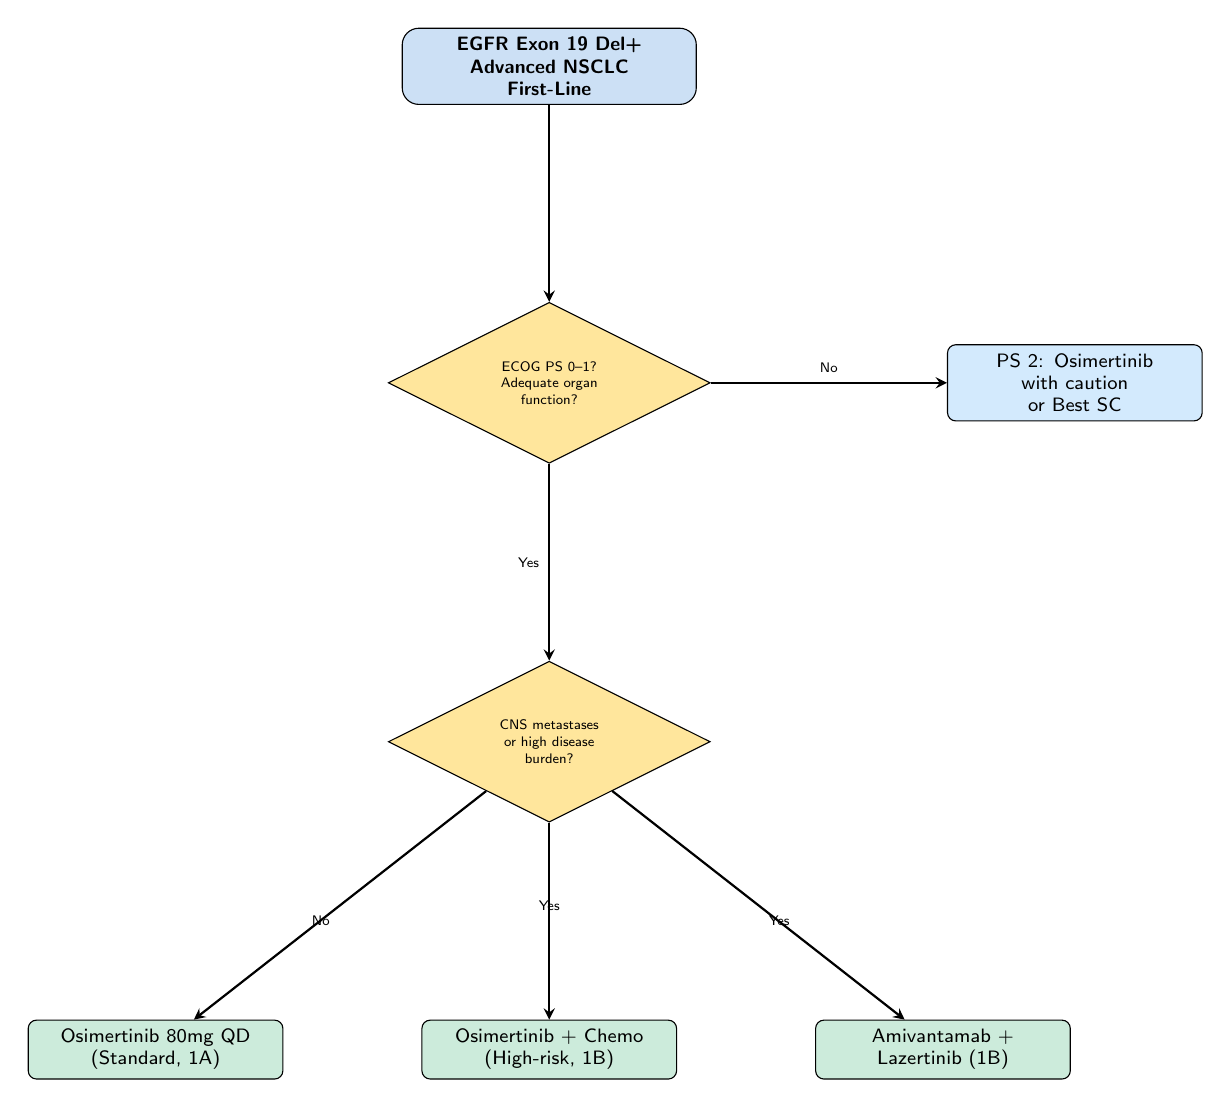
\begin{tikzpicture}[node distance=1.8cm and 3cm, auto,
  startstop/.style={rectangle, rounded corners=6pt, minimum width=3cm, minimum height=0.8cm, text centered, draw=black, fill=headerblue!20, font=\scriptsize\bfseries, text width=3.5cm},
  decision/.style={diamond, minimum width=2.5cm, minimum height=1cm, text centered, draw=black, fill=conditionalyellow!40, font=\tiny, aspect=2, inner sep=0pt, text width=3cm},
  process/.style={rectangle, rounded corners=3pt, minimum width=3cm, minimum height=0.7cm, text centered, draw=black, fill=stronggreen!20, font=\scriptsize, text width=3cm},
  urgent/.style={rectangle, rounded corners=3pt, minimum width=3cm, minimum height=0.7cm, text centered, draw=warningred, line width=1.2pt, fill=warningred!15, font=\scriptsize\bfseries, text width=3cm},
  routine/.style={rectangle, rounded corners=3pt, minimum width=3cm, minimum height=0.7cm, text centered, draw=black, fill=researchblue!20, font=\scriptsize, text width=3cm},
  arrow/.style={thick,->,>=stealth}]

% Entry
\node[startstop] (entry) {EGFR Exon 19 Del+\\Advanced NSCLC\\First-Line};

% Decision 1: Fitness
\node[decision, below=2.5cm of entry] (fit) {ECOG PS 0--1?\\Adequate organ\\function?};

% Decision 2: CNS
\node[decision, below=2.5cm of fit] (cns) {CNS metastases\\or high disease\\burden?};

% Options
\node[process, below=2.5cm of cns, xshift=-5cm] (osim) {Osimertinib 80mg QD\\(Standard, 1A)};
\node[process, below=2.5cm of cns] (combo) {Osimertinib + Chemo\\(High-risk, 1B)};
\node[process, below=2.5cm of cns, xshift=5cm] (amiv) {Amivantamab +\\Lazertinib (1B)};

% PS2 branch
\node[routine, right=3cm of fit] (ps2) {PS 2: Osimertinib\\with caution\\or Best SC};

% Arrows
\draw[arrow] (entry) -- (fit);
\draw[arrow] (fit) -- node[anchor=east, font=\tiny]{Yes} (cns);
\draw[arrow] (fit) -- node[anchor=south, font=\tiny]{No} (ps2);
\draw[arrow] (cns) -- node[anchor=north east, font=\tiny]{No} (osim);
\draw[arrow] (cns) -- node[anchor=south, font=\tiny]{Yes} (combo);
\draw[arrow] (cns) -- node[anchor=north west, font=\tiny]{Yes} (amiv);

\end{tikzpicture}
\end{center}

\subsection{Recommendation for This Patient}

\begin{tcolorbox}[enhanced,colback=stronggreen!8,colframe=stronggreen,
title={\textbf{Recommended First-Line Treatment}},
fonttitle=\bfseries\small,coltitle=black]
{\small
\textbf{Primary Recommendation}: \textbf{Osimertinib 80 mg orally once daily} (GRADE 1A)

\textbf{Rationale for this patient}:
\begin{itemize}
\item EGFR exon 19 deletion confirmed -- strong predictive biomarker for osimertinib response
\item ECOG PS 1 -- fully eligible for osimertinib monotherapy
\item No prior systemic therapy -- standard first-line setting
\item No confirmed brain metastases -- osimertinib provides excellent CNS penetration as prophylaxis
\item No severe hepatic/renal impairment -- standard dosing appropriate
\item Exon 19 deletion subgroup derives greatest benefit from osimertinib (PFS HR 0.38, OS HR 0.68 vs.~1st-gen TKI)
\end{itemize}

\textbf{Alternative Consideration}: If baseline imaging reveals high tumor burden, multiple brain metastases, or \textit{TP53} co-mutation, discuss osimertinib + chemotherapy combination (FLAURA2) as an option, balancing the PFS benefit (25.5 vs.~16.7 months) against increased toxicity (grade $\geq$3 AEs 64\%).

\textbf{Shared Decision-Making Points}:
\begin{itemize}
\item Discuss oral vs.~IV therapy preferences
\item Review expected side effect profile and management strategies
\item Address financial toxicity and insurance coverage
\item Discuss clinical trial options if available
\end{itemize}
}
\end{tcolorbox}

\section{Subsequent Therapy Planning}

\subsection{Progression on Osimertinib}

Upon disease progression on first-line osimertinib, the following workup and treatment options should be considered:

\textbf{Re-biopsy and Resistance Mechanism Assessment}:
\begin{itemize}
\item Tissue biopsy preferred (histologic transformation assessment: SCLC transformation $\sim$5--15\%)
\item Liquid biopsy (ctDNA) for molecular resistance profiling
\item Key resistance mechanisms: \textit{MET} amplification (15--20\%), \textit{EGFR} C797S (7--10\%), HER2 amplification, \textit{BRAF} mutations, SCLC/NSCLC transformation
\end{itemize}

\textbf{Second-Line Options}:
\begin{itemize}
\item \textbf{Osimertinib + Amivantamab}: Emerging data for post-osimertinib progression
\item \textbf{Platinum-pemetrexed chemotherapy}: Standard option (ORR $\sim$30\%, PFS $\sim$5 months)
\item \textbf{Amivantamab + Chemotherapy}: PAPILLON regimen for post-TKI progression
\item \textbf{Antibody-drug conjugates}: HER2-directed (if HER2+), TROP2-directed (investigational)
\item \textbf{Clinical trials}: Strongly encouraged -- novel combinations and next-generation agents
\end{itemize}

\section{Safety and Monitoring}

\subsection{Osimertinib-Specific Monitoring Schedule}

\begin{table}[H]
\centering
\small
\begin{tabular}{p{3.5cm}p{3cm}p{5cm}}
\toprule
\textbf{Assessment} & \textbf{Frequency} & \textbf{Action Threshold} \\
\midrule
CT chest/abdomen & Every 8--12 weeks & RECIST progression $\rightarrow$ re-biopsy \\
Brain MRI & Baseline + PRN & New CNS lesions $\rightarrow$ assess local therapy \\
CBC, CMP, LFTs & Every 3 months & Grade $\geq$3 cytopenia/transaminitis \\
ECG (QTc) & Baseline + PRN & QTc $>$500 ms $\rightarrow$ hold, dose reduce \\
LVEF & Baseline + PRN & LVEF $<$50\% or $\geq$10\% decline $\rightarrow$ hold \\
Skin/nail assessment & Every visit & Grade $\geq$2 $\rightarrow$ topical Rx, dose adjust \\
GI tolerance & Every visit & Grade $\geq$2 diarrhea $\rightarrow$ loperamide, dose adjust \\
\bottomrule
\end{tabular}
\caption{Monitoring schedule for osimertinib therapy}
\end{table}

\subsection{Adverse Event Management}

\begin{tcolorbox}[enhanced,colback=warningred!5,colframe=warningred,
title={\textbf{Critical Safety Alerts}},
fonttitle=\bfseries\small,coltitle=black]
{\small
\begin{itemize}
\item \textbf{ILD/Pneumonitis} (3.9\%): Any new or worsening dyspnea, cough, or fever $\rightarrow$ HOLD osimertinib, CT chest, pulmonology consult. \textbf{Permanently discontinue} if confirmed ILD.
\item \textbf{QTc Prolongation}: Monitor ECG in patients with cardiac risk factors or concomitant QTc-prolonging drugs. Hold if QTc $>$500 ms; resume at reduced dose when $<$481 ms.
\item \textbf{Cardiomyopathy}: Monitor LVEF if cardiac symptoms develop. Hold if LVEF $<$50\% with $\geq$10\% absolute decline.
\item \textbf{Keratitis/Ocular}: Eye pain, photophobia, blurred vision $\rightarrow$ ophthalmology referral.
\end{itemize}
}
\end{tcolorbox}

\section{Clinical Trial Opportunities}

\begin{itemize}
\item \textbf{First-line novel combinations}: Osimertinib + anti-angiogenic agents, osimertinib + immunotherapy (caution: ILD risk)
\item \textbf{Next-generation EGFR TKIs}: Fourth-generation TKIs targeting C797S and other resistance mutations
\item \textbf{Antibody-drug conjugates}: TROP2-directed, HER3-directed agents in first-line combinations
\item \textbf{Recommendation}: Clinical trial enrollment should always be discussed as an option (GRADE R)
\end{itemize}

\section{References}

{\small
\begin{enumerate}
\item Soria JC, et al. Osimertinib in Untreated EGFR-Mutated Advanced Non-Small-Cell Lung Cancer. \textit{N Engl J Med}. 2018;378(2):113-125.
\item Ramalingam SS, et al. Overall Survival with Osimertinib in Untreated, EGFR-Mutated Advanced NSCLC. \textit{N Engl J Med}. 2020;382(1):41-50.
\item Planchard D, et al. Osimertinib with or without Chemotherapy in EGFR-Mutated Advanced NSCLC. \textit{N Engl J Med}. 2023;389(21):1935-1948.
\item Cho BC, et al. Amivantamab plus lazertinib in treatment-naive EGFR-mutated advanced NSCLC (MARIPOSA). \textit{Lancet Oncol}. 2024;25(4):463-476.
\item Soria JC, et al. Dacomitinib versus gefitinib in previously untreated, advanced EGFR+ NSCLC (ARCHER 1050). \textit{Lancet Oncol}. 2018;19(2):227-237.
\item Ramalingam SS, et al. Updated overall survival with dacomitinib versus gefitinib in patients with EGFR+ advanced NSCLC (ARCHER 1050). \textit{J Clin Oncol}. 2020;38(34):4029-4036.
\item NCCN Clinical Practice Guidelines in Oncology: Non-Small Cell Lung Cancer. Version 3.2025.
\item ESMO Clinical Practice Guidelines: Metastatic non-small cell lung cancer. 2024.
\item CSCO Guidelines for Non-Small Cell Lung Cancer. 2024.
\item Hendriks LE, et al. Non-small cell lung cancer: ESMO Clinical Practice Guidelines. \textit{Ann Oncol}. 2024.
\end{enumerate}
}

\vspace{6pt}

\begin{tcolorbox}[colback=highlightgray,colframe=black]
{\small
\textbf{Disclaimer}: This document is intended for use by qualified healthcare professionals as a clinical decision support tool. It does not replace individual clinical judgment. Treatment decisions should be made through shared decision-making between the treating physician and the patient, considering individual patient preferences, comorbidities, and local treatment availability. Evidence and guidelines are subject to change as new data emerge.\\[4pt]
\textbf{Document Classification}: CONFIDENTIAL -- For Professional Use Only\\
\textbf{Prepared}: 2025-06-15 | \textbf{Version}: 1.0 | \textbf{Next Review}: 2025-12-15
}
\end{tcolorbox}

\end{document}
